\documentclass[letterpaper, 12pt]{article}
\usepackage[margin=1in]{geometry}
\usepackage{times}
\usepackage{setspace}
\usepackage{lipsum}
\usepackage{graphicx}
\usepackage{float}
\usepackage[font=footnotesize]{caption}
\graphicspath{ {./} }

\begin{document}
\bibliographystyle{plain}

\begin{titlepage}
    \begin{center}
        \vspace*{1in}
        \Huge{\textbf{Mini Project 2}}
        
        \vspace{0.5in}
        \Large{Noah Schiro}\\
        \Large{Jason Swope}
        
        \vfill
        
        \normalsize{November 24th, 2023}
        
        \vspace{0.5in}
        
        \normalsize{EE456: Introduction to Neural Networks}
        
        \vspace{0.5in}
        
        \normalsize{Pennsylvania State University}
        
    \end{center}
\end{titlepage}

\newpage

\setlength{\parindent}{5ex}
\setstretch{2} 

\section{Introduction}
In this project, we aim to demonstrate the capabilities of a convolutional neural networks (CNN), particularly their efficacy in classification tasks for imagery. For this, we are using the CIFAR-10 dataset. This dataset consists of 60,000 images spread across 10 classes where each image is 32x32x3 (width, height, and channels) in size. For the model, we decided to create our own architecture to see how our model performs against something that has been well optimized for this task (VGG-16, ResNet, or ImageNet for instance).

The objective of this project is to create a balance between inference speed and model accuracy. In embedded applications, computer vision still needs to be heavily optimized in order to run on the target device at reasonable frame rates. Using state of the art architectures such as VGG-16 is not feasible for certain compute platforms if one expects the platform to run at 60 frames-per-second. VGG-16 contains 138 million parameters, leading to extremely slow inference. We will create a smaller model with 150k parameters, while still getting appreciable performance.

We seek to deliver the following:
\begin{enumerate}
\item Plot of training loss over epochs
\item Plot of validation loss over epochs
\item Plot of accuracy on the validation set over each epoch
\item Confusion matrix for our classes (at the end of training)
\item Precision and recall for each class (at the end of training)
\item Associated code to replicate efforts
\end{enumerate}

\section{Implementation}
\subsection{Model architecture}

The model consists of 3 convolutional layers, a flattening step, a feed forward network, and finally a softmax on the output.
\begin{enumerate}
\item Convolutional block 1
    \begin{enumerate}
    \item 2D convolution (3 in-channels, 64 out-channels, kernel size 3, padding 1)
    \item Relu
    \item 2D Maximum pooling
    \end{enumerate}
    
\item Convolutional block 2
    \begin{enumerate}
    \item 2D convolution (64 in-channels, 64 out-channels, kernel size 3, padding 1)
    \item Relu
    \item 2D Maximum pooling
    \end{enumerate}
    
\item Convolutional block 3
    \begin{enumerate}
    \item 2D convolution (64 in-channels, 64 out-channels, kernel size 3, padding 1)
    \item Relu
    \item 2D Maximum pooling
    \end{enumerate}
\item Flatten the tensor
\item Classification step
    \begin{enumerate}
     \item Linear layer (64 dimensional input to 1024 output)
     \item ReLU
     \item Linear layer (1024 dimensional input to 10 classes)
    \end{enumerate}
\item Softmax
\end{enumerate}

\subsection{Data preprocessing}
The data was read in using Pytorch's torchvision library, converted to a tensor, and normalized using 0.5 as the mean and standarad deviation for each channel. In the future, this could be improved by computing the actual mean and standard deviation for the library.

We did not select a train-test split as the CIFAR-10 dataset comes with a seperate training and testing set already.

\subsection{Model training}
The model was trained in a standard fashion, with some notable exceptions. First is the hyperparameters settings:

\begin{itemize}
\item Batch size was set to 64. Such a high batch size seemed to lead to quicker convergence as well as faster processing due to GPU parrallelism.
\item Epochs was set to 50. We observed minimal improvements after 50 epochs.
\item Intial learning rate was set to 0.1. While this seems quick high, we didn't run into any exploding gradient issues with this and it led to extremely quick convergence.
\item Each epoch, we exponentially decayed the learning rate with the following rule \[lr_{e+1} = lr_{e} * 0.95\]
After 50 epochs, our learning rate would be \[0.1 * 0.95^{50} = 0.007694498\]
\end{itemize}

In the interest of time and resources, several strides were also made to decrease the training time. Firstly, a NVIDIA 3060 GPU was deployed as opposed to training with a CPU. The typical optimization that come with using a CUDA enabled card were also used, such as memory pinning and increasing CPU workers in the dataloading step of training.

On top of this, this GPU happens to use the Ampere architecture, which contains tensor cores. These cores should see a 2-3x speed up if we decide to use automatic mixed precision (AMP). This should also decrease our memory requirements and therefore we can increase our batch size (which is typically limited by the VRAM available to you). With these considerations in mind, we did take advantage of AMP optimizations.

At teh end of training, we were able to acheive a training time of 2 minutes and 56 seconds for a model that acheives 72.61\% accuracy.


\section{Results}

The CNN performed very well.  The model reached a validation accuracy of 72.61\% and a validation loss of 1.73609. We found 50 epochs optimized the model without wasting extra compute time. The plots of accuracy vs epochs and loss vs epochs is shown in Figure 1. Figure 1 shows that there is a discrepency between the training and testing dataset, as three is a clear separation between the training and testing datatsets in both accuracy and loss. This incidcates the model is slightly overfitting the training dataset, so randomly choosing training and testing datasets ourselves or using cross-validation might have been advantageous.

\begin{figure}[H]
\centering
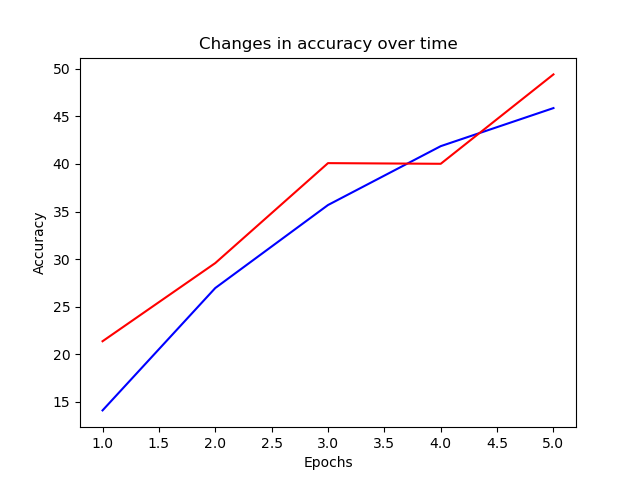
\includegraphics[scale = 0.5]{accuracy}
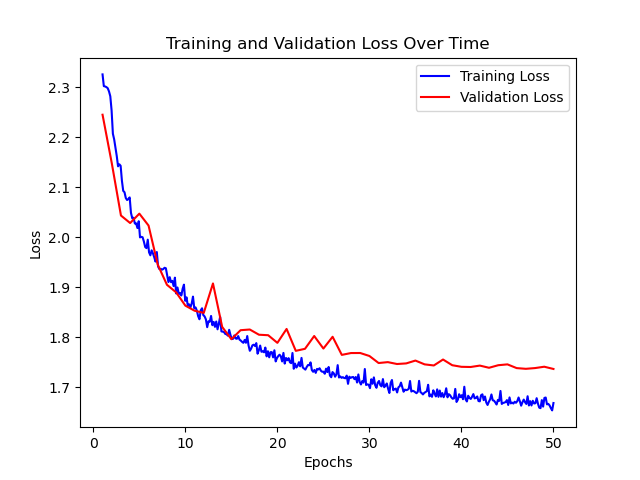
\includegraphics[scale = 0.5]{loss}
\caption{Plot of the accuracy vs epochs (Left) and the plot of the loss vs epochs (Right)}
\end{figure}

The confusion matrix of the model is shown in Figure 2. Correctly classified datapoints appear along the primary diagonal, and Figure 2 shows that the model performed quite well. However, there are some classes that the model struggles to separate, although these classes are logical such as cats and dogs, and ships and airplanes.

\begin{figure}[H]
\centering
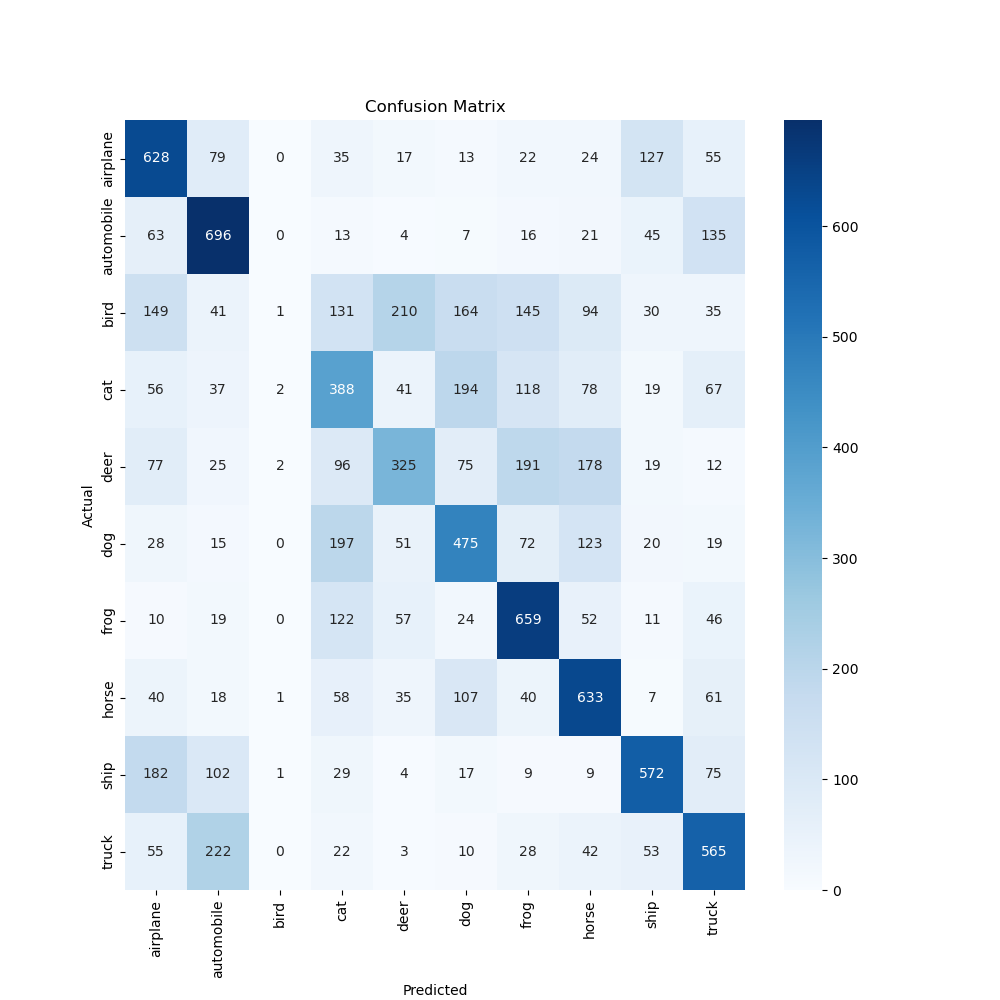
\includegraphics[scale = 0.5]{confusion_matrix}
\caption{Plot of the confusion matrix}
\end{figure}

Looking at some example images and their classifications shown in Figure 3, it appears the model is quite accurate, achieving a confidence of over 98\% on most of the images. However, these example images do show some of the inaccuracies in the model. The model incorrectly classified the frog in the top right, which the model classified as a deer with a decent confidence, which indicates it has learned that deer are brown shapes with green backgrounds. Additionally, the models struggled to accurately predict the automobile in the second row and second coluimn.  It did accurately predict the class, however it only was about 50\% confident in its prediction, which is considerably lower than the confidence levels of the other examples.

\begin{figure}[H]
\centering
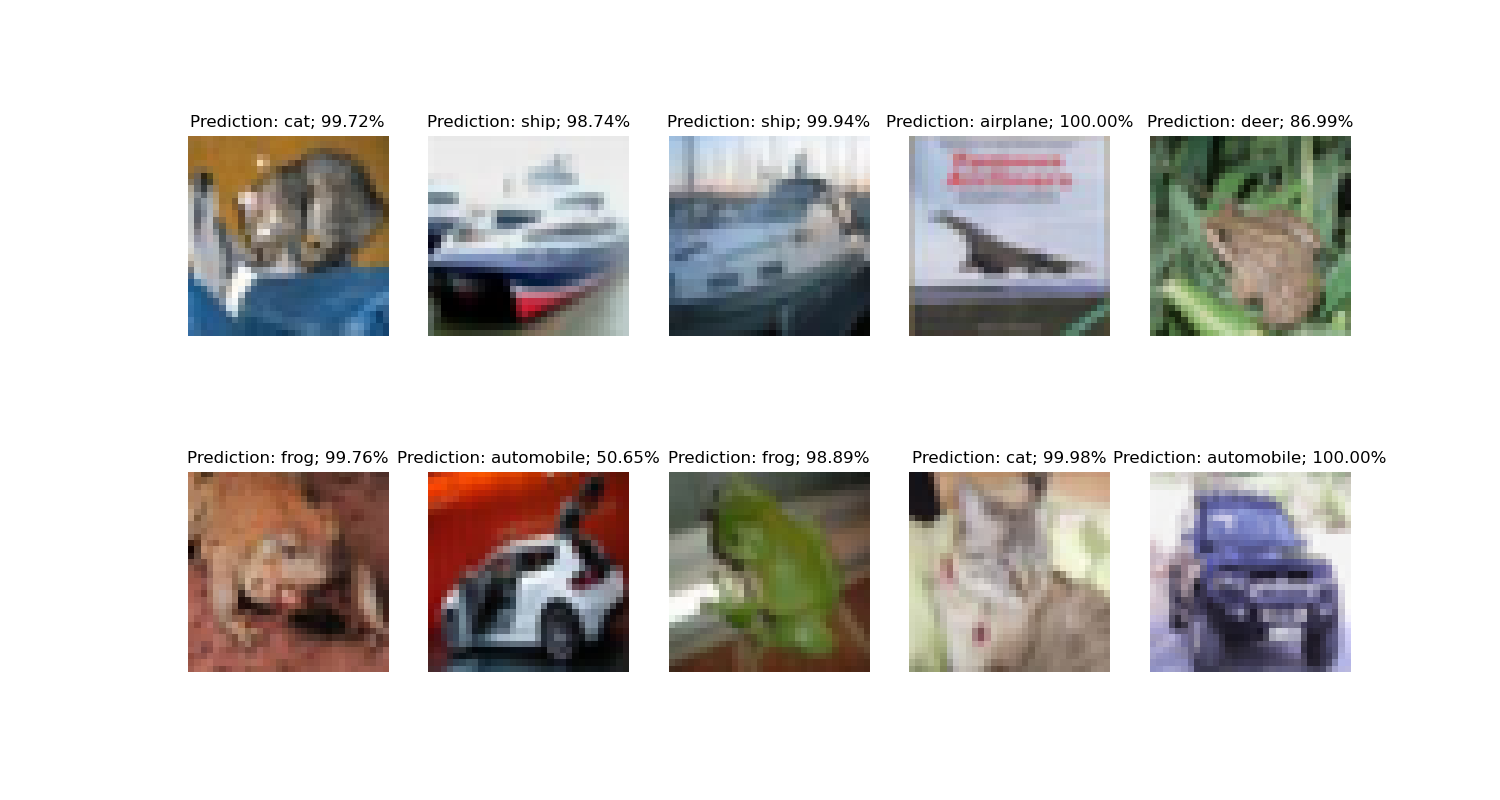
\includegraphics[scale = 0.5]{example_predictions}
\caption{Image of some example images and their classifications}
\end{figure}

The precision and recall  for each class can be seen in Figure 4. The precision and recall for each class are quiet similar, which indicates the model is not prioritizing or leaving behind any of the classes. The best classes are Ships and Automobiles with both precision and recalls above 0.8, and the worst are Cats and Dogs, which have precison and recall below 0.6.

\begin{figure}[H]
\centering
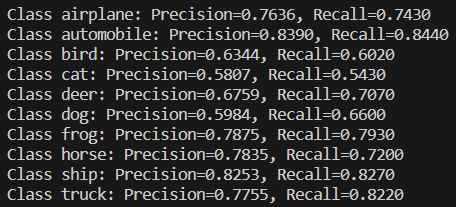
\includegraphics[scale = 0.8]{precision_and_recall}
\caption{Image of the precision and recall for each class}
\end{figure}

\end{document}
